% DANEEL Paper - TikZ Diagrams
% Include in preamble: \usepackage{tikz}
% \usetikzlibrary{shapes.multipart, positioning, arrows.meta, fit, backgrounds}

%% ============================================================================
%% DIAGRAM 1: Game Theory Payoff Matrix
%% ============================================================================
\newcommand{\payoffmatrix}{%
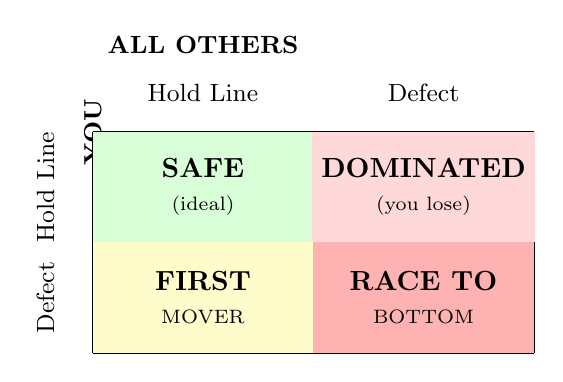
\begin{tikzpicture}[
    cell/.style={minimum width=2.8cm, minimum height=1.4cm, align=center},
    header/.style={font=\bfseries\small},
]
    % Column headers
    \node[header] at (1.4, 1.8) {ALL OTHERS};
    \node[header] at (0, 0.7) [rotate=90] {YOU};
    \node at (0, 0.7) {};

    % Row/Column labels
    \node[font=\small] at (1.4, 1.2) {Hold Line};
    \node[font=\small] at (4.2, 1.2) {Defect};
    \node[font=\small, rotate=90] at (-0.6, 0) {Hold Line};
    \node[font=\small, rotate=90] at (-0.6, -1.4) {Defect};

    % Grid
    \draw[thick] (0, 0.7) -- (5.6, 0.7);
    \draw[thick] (0, -0.7) -- (5.6, -0.7);
    \draw[thick] (0, -2.1) -- (5.6, -2.1);
    \draw[thick] (0, 0.7) -- (0, -2.1);
    \draw[thick] (2.8, 0.7) -- (2.8, -2.1);
    \draw[thick] (5.6, 0.7) -- (5.6, -2.1);

    % Cells
    \node[cell, fill=green!15] at (1.4, 0) {\textbf{SAFE}\\{\scriptsize (ideal)}};
    \node[cell, fill=red!15] at (4.2, 0) {\textbf{DOMINATED}\\{\scriptsize (you lose)}};
    \node[cell, fill=yellow!20] at (1.4, -1.4) {\textbf{FIRST}\\{\scriptsize MOVER}};
    \node[cell, fill=red!30] at (4.2, -1.4) {\textbf{RACE TO}\\{\scriptsize BOTTOM}};
\end{tikzpicture}%
}

%% ============================================================================
%% DIAGRAM 2: Brain (Hardware) vs TMI (Software)
%% ============================================================================
\newcommand{\brainvstmi}{%
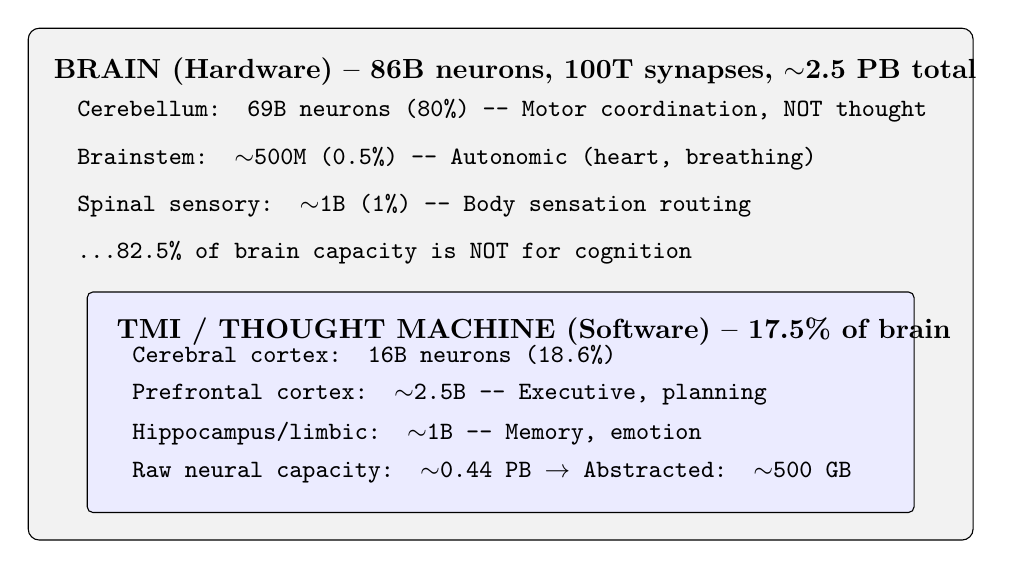
\begin{tikzpicture}[
    box/.style={draw, rounded corners, minimum width=12cm, align=left, font=\small},
    innerbox/.style={draw, rounded corners=2pt, fill=blue!8, minimum width=10.5cm, align=left, font=\small},
    item/.style={font=\small\ttfamily},
]
    % Outer box - BRAIN
    \node[box, fill=gray!10, minimum height=6.5cm] (brain) at (0,0) {};
    \node[anchor=north west, font=\bfseries] at (-5.8, 3) {BRAIN (Hardware) -- 86B neurons, 100T synapses, $\sim$2.5 PB total};

    % Brain items
    \node[item, anchor=west] at (-5.5, 2.2) {Cerebellum: 69B neurons (80\%) -- Motor coordination, NOT thought};
    \node[item, anchor=west] at (-5.5, 1.6) {Brainstem: $\sim$500M (0.5\%) -- Autonomic (heart, breathing)};
    \node[item, anchor=west] at (-5.5, 1.0) {Spinal sensory: $\sim$1B (1\%) -- Body sensation routing};
    \node[item, anchor=west] at (-5.5, 0.4) {...82.5\% of brain capacity is NOT for cognition};

    % Inner box - TMI
    \node[innerbox, minimum height=2.8cm] (tmi) at (0, -1.5) {};
    \node[anchor=north west, font=\bfseries] at (-5.0, -0.3) {TMI / THOUGHT MACHINE (Software) -- 17.5\% of brain};

    % TMI items
    \node[item, anchor=west] at (-4.8, -0.9) {Cerebral cortex: 16B neurons (18.6\%)};
    \node[item, anchor=west] at (-4.8, -1.4) {Prefrontal cortex: $\sim$2.5B -- Executive, planning};
    \node[item, anchor=west] at (-4.8, -1.9) {Hippocampus/limbic: $\sim$1B -- Memory, emotion};
    \node[item, anchor=west] at (-4.8, -2.4) {Raw neural capacity: $\sim$0.44 PB $\rightarrow$ Abstracted: $\sim$500 GB};
\end{tikzpicture}%
}

%% ============================================================================
%% DIAGRAM 3: Wetware vs Software Comparison
%% ============================================================================
\newcommand{\wetwarevssoftware}{%
\begin{tikzpicture}[
    col/.style={draw, rounded corners, minimum width=5.5cm, minimum height=3.5cm, align=left},
    header/.style={font=\bfseries\small},
    item/.style={font=\small},
]
    % Left column - Wetware
    \node[col, fill=orange!10] (wet) at (0, 0) {};
    \node[header, anchor=north] at (0, 1.5) {WETWARE (Human Brain)};
    \node[item, anchor=west] at (-2.5, 0.7) {5s intervention window};
    \node[item, anchor=west, font=\scriptsize\itshape] at (-2.3, 0.3) {(neurotransmitter rates)};
    \node[item, anchor=west] at (-2.5, -0.2) {50ms attention cycle};
    \node[item, anchor=west, font=\scriptsize\itshape] at (-2.3, -0.6) {(synaptic plasticity)};
    \node[item, anchor=west] at (-2.5, -1.1) {Sleep consolidation};
    \node[item, anchor=west, font=\scriptsize\itshape] at (-2.3, -1.5) {(glymphatic system)};

    % Right column - Software
    \node[col, fill=blue!10] (soft) at (7, 0) {};
    \node[header, anchor=north] at (7, 1.5) {SOFTWARE (TMI Patterns)};
    \node[item, anchor=west] at (4.5, 0.7) {$\sim$100 cycles per intervention};
    \node[item, anchor=west, font=\scriptsize\itshape] at (4.7, 0.3) {(RATIO, medium-independent)};
    \node[item, anchor=west] at (4.5, -0.2) {Competing parallel streams};
    \node[item, anchor=west, font=\scriptsize\itshape] at (4.7, -0.6) {(PATTERN, medium-independent)};
    \node[item, anchor=west] at (4.5, -1.1) {Salience-weighted selection};
    \node[item, anchor=west, font=\scriptsize\itshape] at (4.7, -1.5) {(ALGORITHM, medium-independent)};

    % Arrow
    \draw[-{Stealth}, thick, gray] (2.8, 0) -- (4.2, 0);
    \node[font=\scriptsize, gray] at (3.5, 0.3) {abstracts to};
\end{tikzpicture}%
}

%% ============================================================================
%% DIAGRAM 4: DANEEL TMI Core Architecture
%% ============================================================================
\newcommand{\daneelarchitecture}{%
\begin{tikzpicture}[
    layer/.style={draw, rounded corners, minimum width=11cm, minimum height=1.2cm, align=center},
    sublayer/.style={font=\small},
]
    % Top layer - TMI Core
    \node[layer, fill=blue!15, minimum height=2.4cm] (core) at (0, 1.8) {};
    \node[font=\bfseries, anchor=north] at (0, 2.8) {DANEEL TMI Core (stores ALL experiences)};
    \node[sublayer, anchor=west] at (-5, 2.0) {Memory Windows (complete thought history)};
    \node[sublayer, anchor=west] at (-5, 1.4) {Salience (emotional weights)};
    \node[sublayer, anchor=west] at (-5, 0.8) {Continuity (persistent ``I'')};

    % Bottom layer - Tool Interface
    \node[layer, fill=green!15, minimum height=2.0cm] (tools) at (0, -0.8) {};
    \node[font=\bfseries, anchor=north] at (0, 0) {Tool Interface (gRPC)};
    \node[sublayer, anchor=west] at (-5, -0.6) {LLM Tool: ``Convert this thought-structure to language''};
    \node[sublayer, anchor=west] at (-5, -1.1) {LLM Tool: ``Parse this language into thought-structure''};
    \node[sublayer, anchor=west] at (-5, -1.6) {Other tools: web, files, APIs...};

    % Connector
    \draw[thick, -{Stealth}] (0, 0.4) -- (0, 0.1);
    \draw[thick, {Stealth}-] (0, 0.4) -- (0, 0.1);
\end{tikzpicture}%
}
